\documentclass[11pt,a4paper]{article}
\usepackage[margin=1in]{geometry}
\usepackage{hyperref}
\usepackage{enumitem}
\usepackage{graphicx}
\usepackage{xcolor}

% -----------------------------------------------------
% bvraghav-tiet-ucs503p-article.sty
% -----------------------------------------------------

% Variable: Lab Instructor
\makeatletter \newcommand{\BvrSetLabInstructor}[1]{%
  \gdef\Bvr@LabInstructor{#1}}
% default
\newcommand{\Bvr@LabInstructor}{Jhonsy Bansal}
% public accessor
\newcommand{\BvrLabInstructorValue}{\Bvr@LabInstructor}
\makeatother

% Add subtitle
\usepackage{titling}
% -- Set title bold
\pretitle{\begin{center}\bfseries\fontsize{18bp}{18bp}\selectfont}
\makeatletter
\newcommand{\BvrSubtitle}[1]{%
  \posttitle{%
    \par\end{center}
    \begin{center}\large#1\end{center}
    \vskip 0.5em}%
}
\makeatother

\usepackage{tikz}
\usetikzlibrary{positioning, arrows.meta, shapes.geometric}

\usepackage{titlesec}

\titlespacing*{\section}
{0pt}{1.2em}{0.5em}

\titlespacing*{\subsection}
{0pt}{0.8em}{0.4em}

% Hints in the section title(s)
\newcommand{\BvrHint}[1]{%
  {\normalfont\normalsize\itshape\hfill #1}}

% -----------------------------------------------------

\title{SmartCross: Railway Phatak Real-Time Status Web App}

\BvrSetLabInstructor{Jhonsy Bansal}

\BvrSubtitle{%
  Project Proposal for UCS503P  \\
  Submitted to: \BvrLabInstructorValue \\ \bfseries
  Thapar Institute of Engineering and Technology% 
}

\author{
  Sandeep Yadav, CSED%
  \thanks{Roll No: \texttt{1024030312}, %
    Email: \texttt{syadav1\_be24\@thapar.edu}}
  \and 
  Moksh, CSED%
  \thanks{Roll No: \texttt{1024030925}, %
    Email: \texttt{mmoksh\_be24\@thapar.edu}}
  \and 
  Gagandeep Singh, CSED%
  \thanks{Roll No: \texttt{1024030314}, %
    Email: \texttt{gsingh17\_be24\@thapar.edu}}
}

\date{\today}

\begin{document}
\maketitle

\section{Higher-order goal%
  \BvrHint{\ldots secondary framing}}
This project aims to improve commuter safety and reduce time lost at unmanned and manned railway level crossings (``phataks'') by giving nearby residents and commuters real-time visibility into gate status, approaching trains, and alternate routes. While the broader goal is to reduce accidents and unnecessary waiting at railway crossings, the immediate engineering objective is to build a measurable, real-time web application, \textbf{SmartCross}, that fetches live train data, predicts gate closures, and pushes location-aware alerts to users near a phatak.

\section{Time-to-value %
\BvrHint{\ldots primary heuristic}}
\begin{itemize}[leftmargin=0.7cm]
     \item We will deliver functional increments quickly by first implementing live train data ingestion and a static map of nearby phataks, followed by prediction, real-time push alerts, and route suggestions in short development iterations.

    \item We will prioritize a working and measurable system over feature completeness by validating each module (data fetching, prediction, alerting, and the map UI) independently and gradually integrating advanced capabilities such as ETA prediction and alternate-route routing.

    \item Success will be defined by the ability to demonstrate real improvements in alert accuracy, alert lead-time, and reduced unnecessary waiting at phataks through controlled experiments and field-style testing.
\end{itemize}

\section{Problem Statement}

Railway level crossings are a frequent point of congestion, uncertainty, and risk for commuters travelling near railway lines. Gate closure timings are rarely known in advance, and commuters have no way of knowing whether a nearby phatak is open, about to close, or already closed until they physically reach it. Common challenges include:

\begin{itemize}
    \item \textbf{No advance visibility of gate status:} Commuters do not know whether a phatak is open, closing soon, or closed until they arrive, leading to wasted time and unsafe last-moment crossing attempts.

    \item \textbf{Lack of train-approach awareness:} Without live train location data, users cannot anticipate when a gate will close or how long a closure will last.

    \item \textbf{No alternate route guidance:} When a phatak is closed, commuters are rarely offered a nearby alternate route, causing long queues and idle waiting.

    \item \textbf{Fragmented data sources:} Train running status, timetables, and phatak locations exist in separate systems with no unified, location-aware, real-time view for the end user.
\end{itemize}

\textbf{Why this matters now (contextual relevance):} As urban and semi-urban traffic increasingly crosses railway lines, giving commuters real-time, predictive, and location-aware information about phatak status can reduce congestion, prevent risky crossing behaviour, and improve daily commute reliability. Building SmartCross provides practical insight into real-time data pipelines, predictive ETA modelling, and location-based alerting systems.

\section{Proposed Solution %
\BvrHint{\ldots software proposition}}

\subsection{Overview}

The proposed solution is to build \textbf{SmartCross}, a web (and mobile-friendly) application that shows users nearby railway phataks, their live status, train-approaching alerts, and alternate routes. The system continuously ingests live train data, maps trains to the nearest phataks, predicts closure windows, and pushes real-time alerts to users located within a defined radius of a gate.

Unlike a static crossing-timetable display, SmartCross focuses on combining live data ingestion, prediction, and real-time push delivery to give commuters an actionable, up-to-the-minute view of the crossings around them. The system will consist of the following major components, organised into four layers as shown in Figure~\ref{fig:smartcross_architecture}:

\begin{itemize}
    \item \textbf{Data Sources:} A Train Status API supplies live train location, delay, next station, and speed, while Timetable Data supplies train schedules, routes, and frequency.

    \item \textbf{Backend Server:} Consists of a Data Fetcher that polls the Train Status API at regular intervals; a Data Processing \& Mapping module that maps trains to tracks and the nearest phataks; a Prediction Engine that estimates train arrival time at each phatak and predicts closure time; a Gate Status Engine that determines gate state (Open, Closing Soon, Closed, Opening Soon); an Alert Engine that prepares alerts for users within a defined radius; and a Database that stores gates, trains, predictions, users, alerts, and history.

    \item \textbf{Real-Time Communication Layer:} A WebSocket Server pushes real-time status updates to connected clients, and a Notification Service sends push notifications to browser and mobile clients.

    \item \textbf{Web App (User):} A React-based frontend that shows nearby gates and their status, sends alerts when a phatak is closing or opening, displays estimated waiting time, suggests alternate routes, and works within a configurable radius (e.g. 1.5 km).
\end{itemize}

\begin{figure}[h]
\centering

\resizebox{\textwidth}{!}{
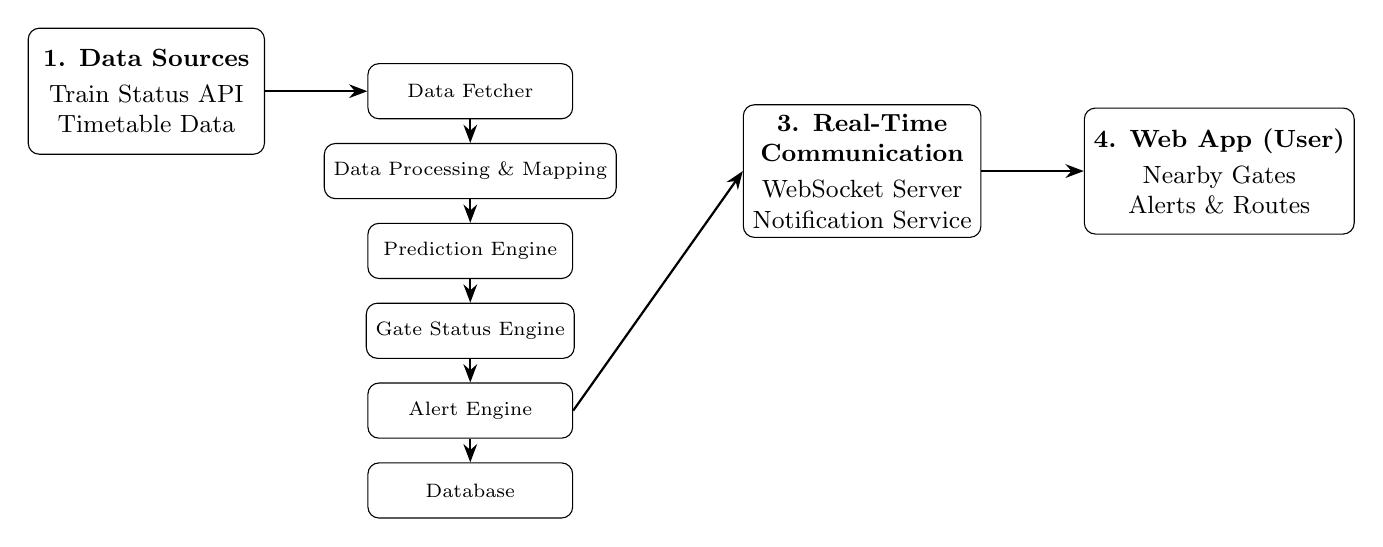
\begin{tikzpicture}[
    node distance=1.1cm and 1.3cm,
    layer/.style={
        rectangle,
        rounded corners,
        draw,
        align=center,
        minimum width=3cm,
        minimum height=1.6cm,
        font=\small
    },
    sub/.style={
        rectangle,
        rounded corners,
        draw,
        align=center,
        minimum width=2.6cm,
        minimum height=0.7cm,
        font=\scriptsize
    },
    arrow/.style={
        thick,
        -{Stealth}
    }
]

% Layer 1: Data Sources
\node[layer] (sources) {
  \textbf{1. Data Sources}\\[2pt]
  Train Status API\\
  Timetable Data
};

% Layer 2: Backend Server
\node[sub, right=of sources] (fetch) {Data Fetcher};
\node[sub, below=0.3cm of fetch] (process) {Data Processing \& Mapping};
\node[sub, below=0.3cm of process] (predict) {Prediction Engine};
\node[sub, below=0.3cm of predict] (gate) {Gate Status Engine};
\node[sub, below=0.3cm of gate] (alertengine) {Alert Engine};
\node[sub, below=0.3cm of alertengine] (db) {Database};

% Layer 3: Real-time comm
\node[layer, right=1.6cm of process] (comm) {
  \textbf{3. Real-Time}\\
  \textbf{Communication}\\[2pt]
  WebSocket Server\\
  Notification Service
};

% Layer 4: Web app
\node[layer, right=of comm] (webapp) {
  \textbf{4. Web App (User)}\\[2pt]
  Nearby Gates\\
  Alerts \& Routes
};

% Arrows
\draw[arrow] (sources) -- (fetch);
\draw[arrow] (fetch) -- (process);
\draw[arrow] (process) -- (predict);
\draw[arrow] (predict) -- (gate);
\draw[arrow] (gate) -- (alertengine);
\draw[arrow] (alertengine) -- (db);

\draw[arrow] (alertengine.east) -- (comm.west);
\draw[arrow] (comm) -- (webapp);

\end{tikzpicture}
}

\caption{High-level architecture of SmartCross showing data sources, backend processing pipeline, real-time communication layer, and the user-facing web app.}

\label{fig:smartcross_architecture}

\end{figure}

\subsection{Core Workflow}

The core workflow of SmartCross follows a complete real-time flow from a train running on the network to a user receiving an actionable alert:

\begin{enumerate}
    \item A train is running, and its live location, speed, and delay are pulled from the Train Status API.

    \item The Data Processing \& Mapping module maps the train to its track and the nearest phatak(s).

    \item The Prediction Engine calculates the estimated time of arrival (ETA) of the train at the mapped phatak.

    \item The Gate Status Engine predicts and updates the gate status (Open, Closing Soon, Closed, Opening Soon) based on the predicted ETA.

    \item The Alert Engine prepares and sends an alert to users located within the defined radius of that phatak.

    \item Users receive the real-time update through the web app or a push notification and can act accordingly, including viewing an alternate route.
\end{enumerate}


\subsection{Operational Constraints}

The project is designed with the following operational constraints:

\begin{itemize}
    \item \textbf{Controlled development environment:} SmartCross will initially operate using a limited set of phataks and a sample/public train-status data feed to allow controlled testing of prediction accuracy and alert delivery.

    \item \textbf{Lightweight implementation:} The system will focus on demonstrating live-data ingestion, prediction, and real-time alerting rather than depending on complex, production-scale railway infrastructure integrations.

    \item \textbf{Open and hosted technology stack:} The implementation will rely on React.js/Tailwind CSS on the frontend, Node.js/Express.js on the backend, MongoDB for storage, Socket.IO for real-time communication, and Google Maps/Mapbox API for maps and routing, deployed on AWS/Render.

    \item \textbf{Focus on correctness and timeliness:} The primary objective is to demonstrate accurate gate-status prediction and timely alert delivery rather than achieving nationwide, production-level coverage.

    \item \textbf{Radius-bound alerting:} Alerts are scoped to users within a configurable radius (e.g. 1.5 km) of a phatak; wider-area or city-scale rollout is future scope.
\end{itemize}

\section{Solution Approach %
\BvrHint{\ldots engineering focus}}

This project follows an engineering-focused approach where the emphasis is on designing, implementing, and evaluating a reliable real-time data pipeline and alerting system. The focus is on building a measurable, real-time web application rather than developing novel train-prediction algorithms. The system will be developed incrementally, with each major module tested independently before integration.

\begin{figure}[ht]
\centering

\resizebox{0.75\textwidth}{!}{
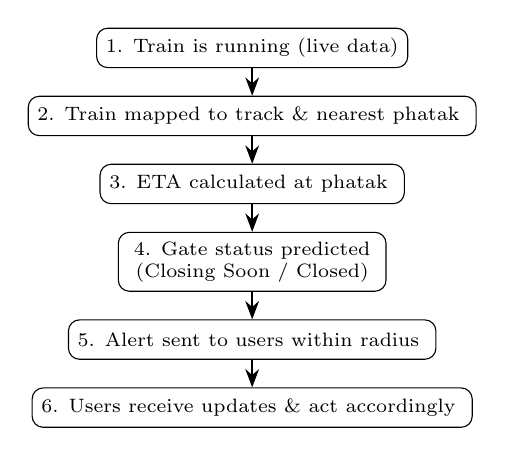
\begin{tikzpicture}[
    box/.style={
        rectangle,
        rounded corners,
        draw,
        minimum width=3.4cm,
        minimum height=0.5cm,
        align=center,
        font=\scriptsize
    },
    arrow/.style={
        thick,
        -{Stealth}
    }
]

% Main flow

\node[box] (train) {1. Train is running (live data)};

\node[box, below=0.35cm of train] (map) {
2. Train mapped to track \& nearest phatak
};

\node[box, below=0.35cm of map] (eta) {
3. ETA calculated at phatak
};

\node[box, below=0.35cm of eta] (status) {
4. Gate status predicted\\
(Closing Soon / Closed)
};

\node[box, below=0.35cm of status] (alert) {
5. Alert sent to users within radius
};

\node[box, below=0.35cm of alert] (receive) {
6. Users receive updates \& act accordingly
};


% Arrows

\draw[arrow] (train)--(map);
\draw[arrow] (map)--(eta);
\draw[arrow] (eta)--(status);
\draw[arrow] (status)--(alert);
\draw[arrow] (alert)--(receive);

\end{tikzpicture}
}

\caption{Real-time flow inside SmartCross from live train data to a user-facing alert.}
\label{fig:smartcross_flow}

\end{figure}

\subsection{Gate Status Prediction}

The gate status logic will be implemented using a small set of well-defined states rather than a single binary open/closed flag.

\begin{itemize}
    \item \textbf{State-based design:} A common gate-status model (Open, Closing Soon, Closed, Opening Soon) will be used consistently across the Prediction Engine, Gate Status Engine, and the frontend UI.

    \item \textbf{ETA-driven predictions:} The Prediction Engine estimates train arrival time at each mapped phatak using live speed, distance, and historical timetable data, and predicts the expected closure window.

    \item \textbf{Configurable alert radius:} The radius within which users receive alerts for a given phatak will be controlled through configuration, allowing tuning without modifying core logic.
\end{itemize}


\subsection{System Architecture}

SmartCross will follow a modular architecture where each responsibility is separated into independent components, as shown in Figure~\ref{fig:smartcross_architecture}.

\begin{itemize}
    \item \textbf{Data Fetcher:} Polls the Train Status API at regular intervals to keep live location, delay, and speed data current.

    \item \textbf{Data Processing \& Mapping:} Maps live trains to tracks and to the nearest phataks using timetable and route data.

    \item \textbf{Prediction Engine:} Estimates train arrival time at each phatak and predicts closure time.

    \item \textbf{Gate Status Engine:} Determines and updates gate status (Open, Closing Soon, Closed, Opening Soon).

    \item \textbf{Alert Engine:} Prepares and dispatches alerts for users within a defined radius of a gate.

    \item \textbf{Real-Time Communication Layer:} A WebSocket Server pushes live updates, and a Notification Service delivers push notifications to browser and mobile clients.
\end{itemize}


\subsection{Concurrency and Real-Time Updates}

Since SmartCross must continuously ingest live train data while simultaneously serving many connected users, concurrency and real-time delivery are core implementation considerations.

\begin{itemize}
    \item Live data polling from the Train Status API will run as an independent background process on a fixed interval.

    \item Gate status recalculation and alert preparation will run independently of client connections so that a slow client cannot block data processing.

    \item Shared state such as gate status, predicted ETAs, and active user sessions will be protected using appropriate synchronization mechanisms and stored centrally in the database.

    \item WebSocket connections will broadcast only the updates relevant to users within a given phatak's radius, to keep the real-time channel efficient.
\end{itemize}

\begin{figure}[ht]
\centering

\resizebox{0.75\textwidth}{!}{
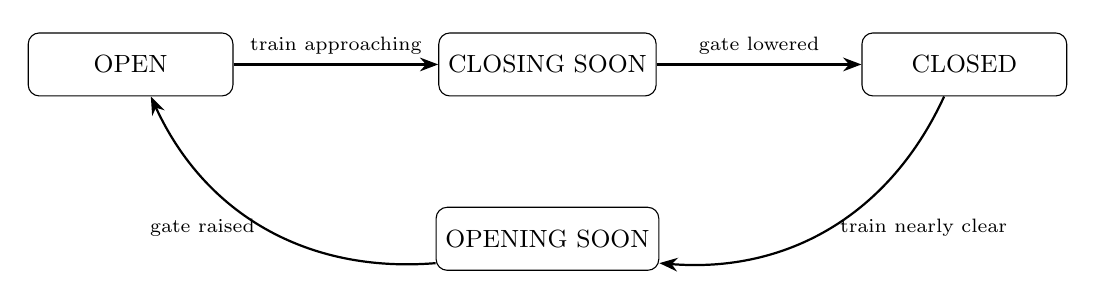
\begin{tikzpicture}[
    state/.style={
        rectangle,
        rounded corners,
        draw,
        minimum width=2.6cm,
        minimum height=0.8cm,
        align=center,
        font=\small
    },
    arrow/.style={
        thick,
        -{Stealth}
    }
]

\node[state] (open) {OPEN};
\node[state, right=2.6cm of open] (closingsoon) {CLOSING SOON};
\node[state, right=2.6cm of closingsoon] (closed) {CLOSED};
\node[state, below=1.4cm of closingsoon] (openingsoon) {OPENING SOON};

\draw[arrow] (open) to node[midway, above]{\scriptsize train approaching} (closingsoon);
\draw[arrow] (closingsoon) to node[midway, above]{\scriptsize gate lowered} (closed);
\draw[arrow] (closed) to[bend left=35] node[midway, right]{\scriptsize train nearly clear} (openingsoon);
\draw[arrow] (openingsoon) to[bend left=35] node[midway, left]{\scriptsize gate raised} (open);

\end{tikzpicture}
}

\caption{Gate status state transition used by SmartCross's Gate Status Engine.}

\label{fig:gate_status_state}

\end{figure}

\subsection{Testing and Performance Evaluation}

The system will be validated through controlled experiments that measure both prediction accuracy and real-time delivery performance.

\begin{itemize}
    \item Test individual components such as train-to-phatak mapping, ETA prediction, gate-status transitions, and alert dispatch independently.

    \item Perform integration testing using a sample of phataks connected to live or simulated train-status data through SmartCross.

    \item Evaluate system behaviour during data feed delays, missing train data, and sudden bursts of nearby users.

    \item Measure performance indicators such as prediction accuracy, alert lead-time, notification delivery latency, and WebSocket update latency.
\end{itemize}


\subsection{CI/CD and Incremental Delivery}

Development will follow an incremental delivery approach to ensure that each stage produces a working system component.

\begin{itemize}
    \item Maintain version control using Git and GitHub with regular commits for each implemented module.

    \item Use automated testing to verify system correctness after changes.

    \item Gradually integrate advanced features such as ETA-based prediction, push notifications, alternate-route suggestions, and history/analytics after the core data-fetching and mapping pipeline is stable.
\end{itemize}

\section{Evaluation Criterion %
\BvrHint{\ldots measurable and attributable}}

The success of SmartCross will be evaluated using measurable prediction accuracy, alert timeliness, and usability metrics directly related to the core system objectives. The evaluation will focus on how effectively the system predicts gate closures and delivers timely, location-relevant alerts.


\subsection{Primary evaluation metric}

\textbf{Alert timeliness and accuracy:} The primary evaluation metric will measure how effectively SmartCross predicts gate status changes and delivers alerts to nearby users before a phatak closes.

\begin{itemize}
    \item \textbf{Target:} Demonstrate that ``Closing Soon'' alerts are delivered with a measurable positive lead-time before actual gate closure, with a low false-alert rate.

    \item \textbf{Attribution:} Measured by comparing predicted closure times against actual/simulated closure times, and by recording notification delivery latency for users within the alert radius.
\end{itemize}


\subsection{Secondary evaluation metrics}

\begin{itemize}
    \item \textbf{Mapping accuracy:} Measure how correctly live trains are mapped to the nearest track and phatak under varying train density.

    \item \textbf{Gate-status transition correctness:} Evaluate how accurately and how quickly the Gate Status Engine transitions between Open, Closing Soon, Closed, and Opening Soon.

    \item \textbf{Real-time delivery latency:} Measure the time between a gate-status change and the corresponding update reaching the WebSocket-connected client and the Notification Service.

    \item \textbf{Route suggestion usefulness:} Assess whether the recommended alternate route, shown when a phatak is closed, offers a meaningfully shorter or faster path than waiting.

    \item \textbf{Observability quality:} Assess whether the stored history of gates, trains, predictions, and alerts accurately supports analytics and later debugging.
\end{itemize}


\subsection{Validation plan}

\begin{itemize}
    \item Deploy SmartCross against a sample set of phataks using a live or simulated Train Status API feed.

    \item Compare predicted ETAs and gate-status transitions against actual/simulated train movement to measure prediction accuracy.

    \item Perform controlled experiments by simulating multiple users within and outside a phatak's alert radius to validate radius-bound alert delivery.

    \item Record system metrics such as alert lead-time, notification latency, WebSocket update latency, and prediction error to validate the effectiveness of the implementation.
\end{itemize}

\section{Scalability %
\BvrHint{\ldots with foresight}}

SmartCross is designed with scalability considerations at both the data-ingestion and system-architecture levels. Although the initial implementation focuses on a limited set of phataks and a single backend instance, the modular design allows future expansion.

\begin{itemize}
    \item \textbf{Phatak scalability:} The database schema for gates, trains, and predictions is designed to support additional phataks being added through configuration and data-mapping rather than code changes.

    \item \textbf{Prediction scalability:} The Prediction Engine's interface allows more sophisticated ETA models (e.g. incorporating historical delay patterns) to be introduced without changing the surrounding pipeline.

    \item \textbf{User scalability:} The WebSocket Server and Notification Service are designed around radius-scoped broadcasting, allowing the system to serve many concurrently connected users without pushing irrelevant updates.

    \item \textbf{Future distributed scaling:} A future version could support multiple regional backend instances and a distributed database. However, this introduces additional challenges such as cross-region data consistency and centralized monitoring, which are outside the scope of the current implementation.
\end{itemize}

\section{Engineering Available Heuristic}

The project follows established engineering practices and existing real-time system concepts rather than attempting to develop new train-prediction algorithms. The objective is to understand, implement, and evaluate proven techniques for live-data ingestion, prediction, and real-time delivery used in real-world systems.

\begin{itemize}
    \item \textbf{Existing real-time patterns:} Well-known techniques such as periodic polling, WebSocket-based push updates, and radius-based geofencing will be implemented and combined instead of designing new distributed protocols.

    \item \textbf{Incremental development:} The system will be developed in stages, starting with basic data fetching and gate-status display and gradually adding prediction, real-time alerts, and route suggestions.

    \item \textbf{Modular engineering approach:} Components such as the Data Fetcher, Data Processing \& Mapping, Prediction Engine, Gate Status Engine, Alert Engine, and Notification Service will remain independent to simplify testing and future improvements.

    \item \textbf{Practical validation:} System behaviour will be evaluated through controlled experiments and measurable benchmarks rather than theoretical assumptions.
\end{itemize}

\section{Project scope and deliverables %
\BvrHint{\ldots iteration-friendly}}

The project scope focuses on developing a functional real-time phatak status web app with live gate tracking, predictive alerts, and route suggestions. Development will follow an incremental approach, where the core data pipeline and status display are implemented first, followed by prediction, real-time alerting, and analytics features.


\subsection{Initial deliverable}

The first iteration will focus on establishing the core functionality of SmartCross:

\begin{itemize}
    \item \textbf{Basic data ingestion:} Implement the Data Fetcher to pull live train location, delay, next station, and speed from the Train Status API at regular intervals.

    \item \textbf{Phatak and train mapping:} Create the Data Processing \& Mapping module and database schema to map trains to tracks and nearest phataks.

    \item \textbf{Basic gate status display:} Implement the Gate Status Engine and a web UI showing nearby gates and their current status (Open, Closing Soon, Closed, Opening Soon).

    \item \textbf{Configurable phatak setup:} Support defining phataks, their coordinates, and basic system settings through a configuration file/database seed.

    \item \textbf{Unit testing and validation:} Test core components such as data fetching, mapping, and gate-status determination.

    \item \textbf{Version control and development workflow:} Maintain the project repository with structured commits and incremental feature integration.
\end{itemize}


\subsection{Subsequent deliverables}

Later iterations will extend the system with prediction, real-time alerting, and analytics capabilities:

\begin{itemize}
    \item \textbf{Prediction Engine:} Implement ETA estimation and closure-time prediction, and evaluate accuracy under different train densities.

    \item \textbf{Real-time communication:} Add the WebSocket Server and Notification Service to push live gate-status updates and alerts to browser/mobile clients.

    \item \textbf{Radius-based alerting:} Implement the Alert Engine to prepare and dispatch alerts for users within a configurable radius of a phatak.

    \item \textbf{Alternate route suggestions:} Integrate Google Maps/Mapbox API to recommend alternate routes when a phatak is closed.

    \item \textbf{Estimated waiting time:} Surface predicted waiting time on the web app based on the Prediction Engine's output.

    \item \textbf{History and analytics:} Store gate, train, prediction, and alert history in the database and expose basic analytics.

    \item \textbf{Benchmarking and evaluation:} Conduct experiments measuring prediction accuracy, alert lead-time, notification latency, and WebSocket update latency.
\end{itemize}

\section{Risks and Mitigations}

\begin{itemize}

    \item \textbf{Live data feed unavailability or inaccuracy:} The Train Status API may have gaps, delays, or inaccuracies that reduce prediction quality.  
    \textbf{Mitigation:} Use a fallback timetable-based estimate when live data is stale or missing, and clearly surface prediction confidence to users.

    \item \textbf{Concurrency and synchronization issues:} Simultaneous data polling, prediction updates, and many connected WebSocket clients may introduce race conditions or inconsistent gate-status states.  
    \textbf{Mitigation:} Design shared components carefully and use synchronization mechanisms such as locks or atomic database updates. Test concurrent behaviour early using controlled workloads.

    \item \textbf{Scope expansion:} Implementing a complete, nationwide phatak-monitoring platform involves several advanced features beyond the semester timeline.  
    \textbf{Mitigation:} Prioritize the core MVP consisting of data ingestion, mapping, gate-status prediction, and radius-based alerting for a limited set of phataks. City-scale or nationwide rollout will remain future scope.

    \item \textbf{Prediction accuracy variability:} ETA and closure-time predictions may vary depending on train speed changes, delays, and incomplete data.  
    \textbf{Mitigation:} Keep prediction logic simple and transparent initially, validate against known train movements, and iterate based on measured error rates.

    \item \textbf{False or missed alerts:} Incorrect gate-status predictions could lead to false ``Closing Soon'' alerts or missed closures, reducing user trust.  
    \textbf{Mitigation:} Evaluate alert precision/recall carefully before enabling automatic push notifications, and allow a manual/community-reported override for known-incorrect statuses.

    \item \textbf{Route-suggestion feature affecting core progress:} Building maps and alternate-route integration may consume time needed for the core data pipeline and alerting.  
    \textbf{Mitigation:} Develop route suggestions only after the core status-tracking and alerting components are stable, using already available Maps APIs.

    \item \textbf{Security and privacy limitations:} Location-based alerting involves user location data that requires careful handling.  
    \textbf{Mitigation:} Clearly define the project as an educational implementation, minimize stored location data, and avoid persisting precise user location beyond what is needed for radius-based alerting.

\end{itemize}


\section{Summary}

This project proposes the development of SmartCross, a real-time railway phatak status web application designed to give commuters visibility into nearby gate status, train-approach alerts, and alternate routes. The system focuses on live data ingestion, predictive gate-status modelling, radius-based real-time alerting, and route suggestions through a modular engineering approach.

The project emphasizes measurable evaluation through controlled experiments involving prediction accuracy, alert lead-time, notification latency, and real-time update delivery. By implementing established real-time system concepts such as periodic data polling, WebSocket-based push updates, and geofenced alerting, SmartCross aims to provide practical understanding of how modern location-aware, real-time systems handle prediction, reliability, and scalability challenges.

The project remains focused on engineering implementation and evaluation rather than developing novel train-prediction algorithms. Its contribution lies in building a functional, measurable, and extensible application that demonstrates the principles behind real-world, real-time public-safety and commuter-information systems.

\end{document}
